\documentclass[12pt,reqno,a4paper]{amsart}
\usepackage{amsmath,amssymb,amsthm,amsfonts}
\usepackage{tikz}
\usetikzlibrary{graphs, graphs.standard}
\tikzset{
	modal/.style={>=stealth’,shorten >=1pt,shorten <=1pt,auto,node distance=1.5cm,
		semithick},
	world/.style={circle, draw,minimum size=.1cm,fill=gray!15},
	point/.style={circle,draw,inner sep=0.3mm,fill=black},
	circ/.style={circle,draw,inner sep=0.1mm,fill=white},
	reflexive above/.style={->,loop,looseness=7,in=120,out=60},
	reflexive below/.style={->,loop,looseness=7,in=240,out=300},
	reflexive left/.style={->,loop,looseness=7,in=150,out=210},
	reflexive right/.style={->,loop,looseness=7,in=30,out=330}
}
\usetikzlibrary{shapes}
\usetikzlibrary{plotmarks}
\usetikzlibrary{arrows}
\usetikzlibrary{positioning}

\begin{document}

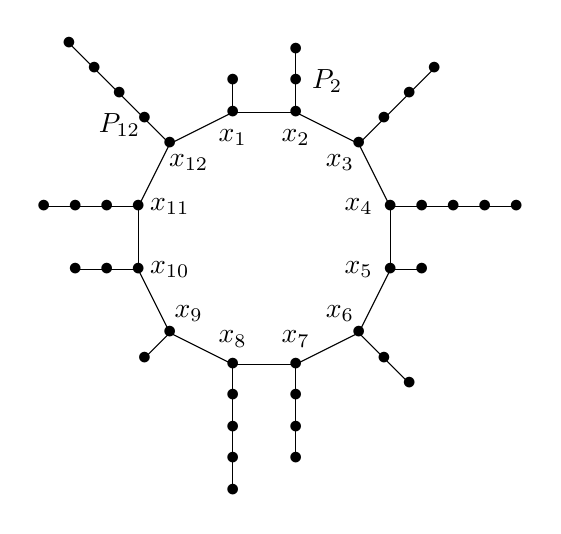
\begin{tikzpicture}[scale=0.8]
	%%%%%%%%%%%%%%%%%%%%%%%%%%%%%%%%%%%%%%%%%%%
	\draw[black,] (-0.5,2) -- (0.5,2);
	\draw[black,] (-0.5,2) -- (-0.5,2.5);
	
	\draw[black,] (0.5,2) -- (1.5,1.5);
	\draw[black,] (0.5,2) -- (0.5,3);
	
	\draw[black,] (1.5,1.5) -- (2,0.5);
	\draw[black,] (1.5,1.5) -- (2.7,2.7);
	
	\draw[black,] (2, 0.5) -- (2, -0.5);
	\draw[black,] (2, 0.5) -- (4,0.5);
	
	\draw[black,] (2, -0.5) -- (1.5, -1.5);
	\draw[black,] (2, -0.5) -- (2.5,-0.5);
	
	\draw[black,] (1.5, -1.5) -- (0.5, -2);
	\draw[black,] (1.5, -1.5) -- (2.3, -2.3);
	
	\draw[black,] (0.5,-2) -- (-0.5,-2);
	\draw[black,] (0.5, -2) -- (0.5, -3.5);
	
	\draw[black,] (-0.5,-2) -- (-1.5,-1.5);
	\draw[black,] (-0.5, -2) -- (-0.5, -4);
	
	\draw[black,] (-1.5,-1.5) -- (-2,-0.5);
	\draw[black,] (-1.5,-1.5) -- (-1.9, -1.9);
	
	\draw[black,] (-2, -0.5) -- (-2, 0.5);
	\draw[black,] (-2, -0.5) -- (-3, -0.5);
	
	\draw[black,] (-2, 0.5) -- (-1.5, 1.5);
	\draw[black,] (-2, 0.5) -- (-3.5, 0.5);
	
	\draw[black,] (-1.5, 1.5) -- (-0.5, 2);
	\draw[black,] (-1.5, 1.5) -- (-3.1, 3.1);
	
	\draw (-0.5,2) node {$\bullet$};
	\draw (-0.5,1.6) node {$x_{1}$};
	\draw (-0.5,2.5) node {$\bullet$};
	
	\draw (0.5,2) node {$\bullet$};
	\draw (0.5,1.6) node {$x_{2}$};
	\draw (0.5,2.5) node {$\bullet$};
	\draw (1,2.5) node {$P_{2}$};
	\draw (0.5,3) node {$\bullet$};
	
	\draw (1.5,1.5) node {$\bullet$};
	\draw (1.2,1.2) node {$x_{3}$};
	\draw (1.9,1.9) node {$\bullet$};
	\draw (2.3,2.3) node {$\bullet$};
	\draw (2.7,2.7) node {$\bullet$};
	
	\draw (2,0.5) node {$\bullet$};
	\draw (1.5,0.5) node {$x_{4}$};
	\draw (2.5,0.5) node {$\bullet$};
	\draw (3,0.5) node {$\bullet$};
	\draw (3.5,0.5) node {$\bullet$};
	\draw (4,0.5) node {$\bullet$};
	
	\draw (2,-0.5) node {$\bullet$};
	\draw (1.5,-0.5) node {$x_{5}$};
	\draw (2.5,-0.5) node {$\bullet$};
	
	\draw (1.5,-1.5) node {$\bullet$};
	\draw (1.2,-1.2) node {$x_{6}$};
	\draw (1.9,-1.9) node {$\bullet$};
	\draw (2.3,-2.3) node {$\bullet$};
	
	\draw (0.5,-2) node {$\bullet$};
	\draw (0.5,-1.6) node {$x_{7}$};
	\draw (0.5,-2.5) node {$\bullet$};
	\draw (0.5,-3) node {$\bullet$};
	\draw (0.5,-3.5) node {$\bullet$};
	
	\draw (-0.5,-2) node {$\bullet$};
	\draw (-0.5,-1.6) node {$x_{8}$};
	\draw (-0.5,-2.5) node {$\bullet$};
	\draw (-0.5,-3) node {$\bullet$};
	\draw (-0.5,-3.5) node {$\bullet$};
	\draw (-0.5,-4) node {$\bullet$};
	
	\draw (-1.5,-1.5) node {$\bullet$};
	\draw (-1.2,-1.2) node {$x_{9}$};
	\draw (-1.9,-1.9) node {$\bullet$};
	
	\draw (-2,-0.5) node {$\bullet$};
	\draw (-1.5,-0.5) node {$x_{10}$};
	\draw (-2.5,-0.5) node {$\bullet$};
	\draw (-3,-0.5) node {$\bullet$};
	
	\draw (-2,0.5) node {$\bullet$};
	\draw (-1.5,0.5) node {$x_{11}$};
	\draw (-2.5,0.5) node {$\bullet$};
	\draw (-3,0.5) node {$\bullet$};
	\draw (-3.5,0.5) node {$\bullet$};
	
	\draw (-1.5,1.5) node {$\bullet$};
	\draw (-1.2,1.2) node {$x_{12}$};
	\draw (-1.9,1.9) node {$\bullet$};
	\draw (-2.3,2.3) node {$\bullet$};
	\draw (-2.3,1.8) node {$P_{12}$};
	\draw (-2.7,2.7) node {$\bullet$};
	\draw (-3.1,3.1) node {$\bullet$};
\end{tikzpicture}

\end{document}